\section{Characterizing Transnational Detours}
\label{datasets}
In this section, we describe our measurement methods, the challenges in
conducting them, and our findings concerning the transnational detours
of default Internet paths.

\subsection{Measurement Approach and Challenges}
\label{pipeline}

\paragraph{Overview of approach}
Figure~\ref{fig:pipeline1} shows the process that we use to discover end-to-end
Internet paths from our respective vantage points to various domains. We first use
VPNs
to establish various vantage points in the countries of interest; then, we use 
{\tt curl} to download corresponding webpages for each of those popular domains,
including all subdomains that are embedded in the site's top-level webpage (1,2). We extract
all of these domain names (3) and resolve them to their corresponding IP addresses (4);
we then perform traceroutes to each of those IP addresses (5).
Figure~\ref{fig:analysis_pipeline} describes how we translate an IP-level traceroute
to a country-level path. We geolocate each IP address, removing unknown hops; we
then de-duplicate the country-level path. Although it is seemingly straightforward,
this approach entails a number of limitations and caveats, which we describe in
the
rest of this section.
%JEN: repetitive
%Using traceroutes to measure
%transnational detours is new; prior work used BGP routing tables to
%\textit{infer} country-level paths~\cite{karlin2009nation}.  

\subsubsection{Resource Limitations}
\label{resource_limits}

We currently focus our measurements on five countries due to resource limitations.
The iPlane~\cite{madhyastha2006iplane} and Center for Applied Internet Data
Analysis (CAIDA)~\cite{caida} projects maintain large repositories of
traceroute data, neither of which are suitable for our study.   iPlane has
historical data as far back as 2006. Unfortunately, because iPlane uses
PlanetLab~\cite{PlanetLab} nodes, which are primarily hosted on the Global
Research and Education Network (GREN), iPlane measurements are not be
representative of typical Internet users' traffic
paths~\cite{banerjee2004interdomain}.  CAIDA runs traceroutes from different
vantage points around the world to randomized destination IP addresses that
cover all /24s; in contrast, we focus on paths to popular websites from a
particular country.

Instead, we run active measurements that better represent paths of a typical Internet user. To do so, we run
DNS and traceroute measurements from RIPE Atlas probes, which are hosted
all around the world in many different types of networks, including home
networks~\cite{ripe_atlas}.  RIPE Atlas probes can use the local DNS
resolver, which give us the best estimate of the traceroute
destination.  

Conducting measurements from a RIPE Atlas probe costs a certain
amount of ``credits'', which restricts the number of measurements that we
can run.  RIPE Atlas also imposes rate limits on the number of
concurrent measurements and the number of credits that an individual
user can spend per day.  We address these challenges in two ways: (1)~we
reduce the number of necessary measurements we must run on RIPE Atlas
probes by conducting traceroute measurements to a single IP address in
each /24 (as opposed to all IP addresses returned by DNS) because all IP
addresses in a /24 belong to the same AS, and should therefore be
located in the same geographic area; (2)~we use a different method---VPN
connections---to obtain a vantage point within a foreign country, which
is still representative of an Internet user in that country.

\subsubsection{Path Asymmetry}
\label{path_sym}

The reverse path (i.e., the path from the server to the client) is just as important as (and often different from) the
forward path.   Previous work has shown that paths between Internet endpoints
are often asymmetric~\cite{he2005routing}.  Most work on path asymmetry has
been done at the AS level~\cite{paxson1997end,gao2001inferring,he2005routing,he2004quantifying}, but not at the country level; our measurements can
consider only the forward path (from client to domain or relay), not the
reverse path from the domain or relay to the client.

We also (separately)
measured path asymmetry at the country granularity. If country-level paths
were symmetric, then the results of our measurements would be representative
of the forward {\it and} reverse paths. If the country-level paths are
asymmetric, then our measurement results only provide a lower bound on the
number of countries that traffic between two endpoints may traverse.  Using
100 RIPE Atlas probes and eight Amazon EC2 instances,
we ran traceroute measurements from every probe to every EC2 instance and from
every EC2 instance to every probe\footnote{The EC2 instances were located in the United States, Brazil, 
Canada, Ireland, Germany, Japan, Australia, and Singapore.}.  After mapping the IP addresses to countries, we
analyzed the paths for symmetry.  First, we compared the set of countries on
the forward path to the set of countries on the reverse path; we found that about 30\% of the 
paths were symmetric at the country level.  We compared the number of countries on the forward and
reverse paths to determine how many reverse paths were a subset of the
respective forward path; this situation occurred for 55\% of the paths. This
level of asymmetry suggests that our results are a lower bound on how
many countries transit a client's path. It also suggests that
while providing lower bounds on transnational detours is feasible, designing
systems to {\em completely} prevent these detours on both forward and reverse
paths is challenging. If tools that shed light on the reverse path
between endpoints (\eg, Reverse Traceroute~\cite{katz2010reverse}) see more widespread deployment,
the characterizations and avoidance techniques that we develop in this paper could
be extended to include reverse paths.

\subsubsection{Traceroute Origin and Destination Selection}

Each country hosts 75 to several hundred RIPE Atlas probes.  Because of resource
restrictions, we could not use all of the probes in each country.  We
selected the set of probes that had unique ASes in the country to get
the widest representation of origination (starting) points.

To determine how many destinations are representative of the popular sites that 
client's access, we first compare the country-level paths from a small set of vantage 
poitns to the Alexa Top 100 domains 
 and to the Alexa Top 1000 domains.  The proportion of paths that transited (and
ended in) each country are similar in both cases; the paths to the top 1000
domains exhibit a longer tail of countries that transit or host content,
likely because these domains are less popular and therefore hosted in more
obscure locations. Otherwise, the results are similar.  This comparison can be 
seen in Figure \ref{fig:compare_alexas}.  Therefore, we used the Alexa Top 100 
domains in each of the respective countries as our destinations, as well as the third-party 
domains that are requested as part of an original web request. 

\begin{figure}[t]
\centering
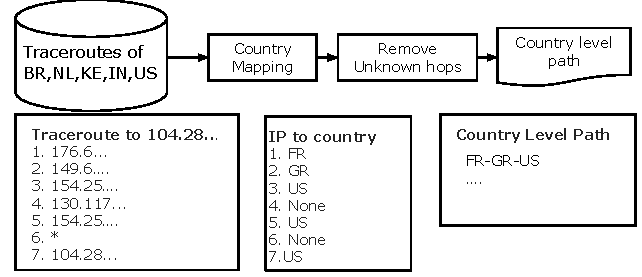
\includegraphics[width=.5\textwidth]{Analysis-Pipeline1}
\caption{Mapping country-level paths from traceroutes.}
\label{fig:analysis_pipeline}
\end{figure}

To obtain the third-party domains that are hosted on each popular website, we
use {\tt curl} to retrieve the homepage for each respective domain from within
the country that is hosting the vantage point in question.  RIPE Atlas probes
do not support these types of Web requests; instead, we establish a VPN
connection within each of these countries to {\tt curl} each domain and
extract the third-party domains; we {\tt curl} from the client's location in
case web sites are customizing content based on the region of the client.

\begin{figure}[t]
\centering
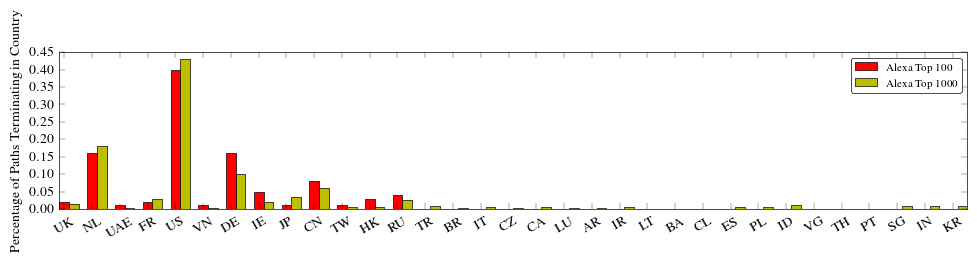
\includegraphics[width=.5\textwidth]{compare_100_100}
\caption{Comparison of path endpoints between the Alexa Top 100 and the Alexa Top 1000.}
\label{fig:compare_alexas}
\end{figure}

\subsubsection{Country Mapping}
\label{c_map}

Accurate IP geolocation is challenging~\cite{poese2011ip,katz2006towards,eriksson2010learning,gill2010dude,hu2012towards,guo2009mining,eriksson2012posit}. We use MaxMind's
geolocation service to map IP addresses to their respective
countries~\cite{maxmind}. Unfortunately, this database is known to contain inaccuracies,
particularly for IP addresses that correspond to Internet infrastructure, as opposed
to end hosts.  Fortunately, previous work has found that
geolocation at a country-level granularity is more accurate than at
finer granularity~\cite{huffaker2011geocompare}.  In light of these
concerns, we post-processed our IP to country mapping; Figure~\ref{fig:analysis_pipeline} shows an example of this
post-processing.  The method starts with removing all IP addresses that resulted in a `None' response when
querying MaxMind, which causes our results to provide a conservative
estimate of the number of countries that paths traverse. It is important
to note that removing `None' responses will \textit{always} produce a
conservative estimate.
%JEN: removed to deemphasize surveillance as the primary interest
%, and therefore we are \textit{always}
%underestimating the amount of potential surveillance.   

\subsection{Results}


%%%% ADD THIS TO datasets.tex
\newcolumntype{d}[1]{D{.}{.}{#1}}
\newcommand{\headrow}[1]{\multicolumn{1}{c}{\adjustbox{angle=45,lap=\width-0.5em}{#1}}}
\newcolumntype{P}[1]{>{\raggedright\arraybackslash}p{#1}}
\newcommand{\ra}[1]{\renewcommand{\arraystretch}{#1}}
\begin{table}[t]
\centering
\ra{1}
\resizebox{\columnwidth}{!}{%
\begin{tabular}{@{}ld{3.2}d{3.2}d{3.2}d{3.2}d{3.2}@{}}
%\multicolumn{1}{l}{}    & \headrow{Host} & \headrow{Transit} & \headrow{Host} & \headrow{Transit} &\headrow{Host} &\headrow{Transit} &\headrow{Host}   &\headrow{Transit} &\headrow{Host}  &\headrow{Transit} \\
\textit{Terminating in Country} 
   & \headrow{Brazil}  & \headrow{Netherlands}   & \headrow{India} & \headrow{Kenya} & \headrow{United States}\\
\toprule
Brazil             &.169    &\multicolumn{1}{r}{-}     &\multicolumn{1}{r}{-}    &\multicolumn{1}{r}{-}  &\multicolumn{1}{r}{-} \\ \midrule
Canada             &.001    &.007     &.015      &.006       &\multicolumn{1}{r}{-}  \\
United States      &\cellcolor[HTML]{F7BE81}.774    &\cellcolor[HTML]{F7BE81}.454      &\cellcolor[HTML]{F7BE81}.629      &\cellcolor[HTML]{F7BE81}.443        &\cellcolor[HTML]{F7BE81}.969    \\ \midrule
France             &.001    &.022      &.009      &.023       &.001 \\
Germany            &.002    &.013      &.014      &.028       &.001  \\
Great Britain      &\multicolumn{1}{r}{-}  &.019     &.021     &.032       &.002 \\
Ireland            &.016    &.064      &.027       &.108       &.001   \\
Netherlands        &.013    &\cellcolor[HTML]{F7BE81}.392      &\cellcolor[HTML]{F7BE81}.101      &\cellcolor[HTML]{F7BE81}.200      &.024  \\
Spain              &.001    &\multicolumn{1}{r}{-}     &\multicolumn{1}{r}{-}    &\multicolumn{1}{r}{-}     &\multicolumn{1}{r}{-}    \\ \midrule
Kenya              &\multicolumn{1}{r}{-}        &\multicolumn{1}{r}{-}    &\multicolumn{1}{r}{-}    &.022        &\multicolumn{1}{r}{-}  \\
Mauritius          &\multicolumn{1}{r}{-}      &\multicolumn{1}{r}{-}    &\multicolumn{1}{r}{-}   &.004       &\multicolumn{1}{r}{-}  \\
South Africa       &\multicolumn{1}{r}{-}       &\multicolumn{1}{r}{-}     &\multicolumn{1}{r}{-}  &.021       &\multicolumn{1}{r}{-}  \\ \midrule
United Arab Emirates &\multicolumn{1}{r}{-}     &\multicolumn{1}{r}{-}     &\multicolumn{1}{r}{-}   &.011        &\multicolumn{1}{r}{-}  \\
India              &\multicolumn{1}{r}{-}      &\multicolumn{1}{r}{-}     &.053    &.002        &\multicolumn{1}{r}{-}  \\
Singapore          &\multicolumn{1}{r}{-}       &.002     &\cellcolor[HTML]{F7BE81}.103      &.027       &\multicolumn{1}{r}{-} \\\hline
\end{tabular}
}
\caption{Fraction of paths that terminate in each country by default.}
\label{tab:host}
\end{table}

\begin{table}[t]
\centering
\ra{1}
\resizebox{\columnwidth}{!}{%
\begin{tabular}{@{}ld{3.2}d{3.2}d{3.2}d{3.2}d{3.2}@{}}
%\multicolumn{1}{l}{}    & \headrow{Host} & \headrow{Transit} & \headrow{Host} & \headrow{Transit} &\headrow{Host} &\headrow{Transit} &\headrow{Host}   &\headrow{Transit} &\headrow{Host}  &\headrow{Transit} \\

\textit{Transiting Country}    & \headrow{Brazil}  & \headrow{Netherlands}   & \headrow{India} & \headrow{Kenya} & \headrow{United States}\\ \toprule
Brazil              &1.00       &\multicolumn{1}{r}{-}   &\multicolumn{1}{r}{-}     &\multicolumn{1}{r}{-}     &\multicolumn{1}{r}{-} \\ \midrule
Canada                &.013       &.007     &.016       &.008      &.081 \\
United States        &\cellcolor[HTML]{F7BE81}.844        &\cellcolor[HTML]{F7BE81}.583     &\cellcolor[HTML]{F7BE81}.715      &\cellcolor[HTML]{F7BE81}.616       &\cellcolor[HTML]{F7BE81}1.00 \\ \midrule
France                 &.059     &.102      &.104       &.221      &.104 \\
Germany                 &.005       &.050    &.032      &.048      &.008 \\
Great Britain                &.024       &\cellcolor[HTML]{F7BE81}.140     &\cellcolor[HTML]{F7BE81}.204      &\cellcolor[HTML]{F7BE81}.500      &.006 \\
Ireland                &.028       &.106      &.031     &.133      &.006 \\
Netherlands                 &.019        &1.00      &.121      &\cellcolor[HTML]{F7BE81}.253      &.031 \\
Spain                  &.176       &.004     &\multicolumn{1}{r}{-}     &\multicolumn{1}{r}{-}      &\multicolumn{1}{r}{-} \\ \midrule
Kenya                 &\multicolumn{1}{r}{-}       &\multicolumn{1}{r}{-}    &\multicolumn{1}{r}{-}      &1.00      &\multicolumn{1}{r}{-} \\
Mauritius                  &\multicolumn{1}{r}{-}       &\multicolumn{1}{r}{-}     &\multicolumn{1}{r}{-}      &\cellcolor[HTML]{F7BE81}.322       &\multicolumn{1}{r}{-} \\
South Africa                 &\multicolumn{1}{r}{-}        &\multicolumn{1}{r}{-}    &\multicolumn{1}{r}{-}     &\cellcolor[HTML]{F7BE81}.334       &\multicolumn{1}{r}{-} \\ \midrule
United Arab Emirates                  &\multicolumn{1}{r}{-}        &\multicolumn{1}{r}{-}    &\multicolumn{1}{r}{-}     &.152       &\multicolumn{1}{r}{-} \\
India               &\multicolumn{1}{r}{-}    &\multicolumn{1}{r}{-}    &1.00     &.058     &\multicolumn{1}{r}{-} \\
Singapore                 &\multicolumn{1}{r}{-}        &.002     &\cellcolor[HTML]{F7BE81}.270       &.040       &.003 \\ \midrule
\end{tabular}
}
\caption{Fraction of paths that each country transits by default.}
\label{tab:transit}
\end{table}


Table~\ref{tab:host} shows five of the countries that we studied along the top
of the table and the countries that host their content along in each row.  A
``-'' represents the case where no paths ended in that country. For example,
the United States is the endpoint of 77.4\% of the paths that originate in
Brazil, and no Brazilian paths terminated in South Africa.
Table~\ref{tab:transit} shows the fraction of paths that transit (or end in)
certain countries, with a row for each country that is transited.  We report 
on measurements conducted on January 31, 2016, and we are continuing to run 
these measurements and publish the data.\footnote{We have published our data 
to an anonymized repository at: \url{https://bitbucket.org/ransom_research/data/}}

\begin{finding}[Hosting Diversity] About half of the top domains in each of
the five countries studied are hosted in a single country.  The other half are
located in two or more different countries. \end{finding} 

\noindent Hosting diversity reveals how many unique
countries host a domain.  The more countries host a domain, the greater the
likelihood that a client can find a path to that site that avoids a certain
country. As a separate measurement experiment, we queried DNS from 26 vantage points around the world, in
geographically diverse locations. We then mapped the IP addresses in the DNS
responses to countries to determine how many unique countries host a domain.
Figure~\ref{fig:host_diversity} shows the fraction of domains that are hosted
in different numbers of countries; we can see two common hosting cases:
(1)~CDNs and (2)~a single hosting country.  This shows that many domains are
hosted in a single unique country, which leads us to our next analysis---where
are these domains hosted, and which countries are traversed on the way to
reach these locations.

%\begin{figure}[t]
%\centering
%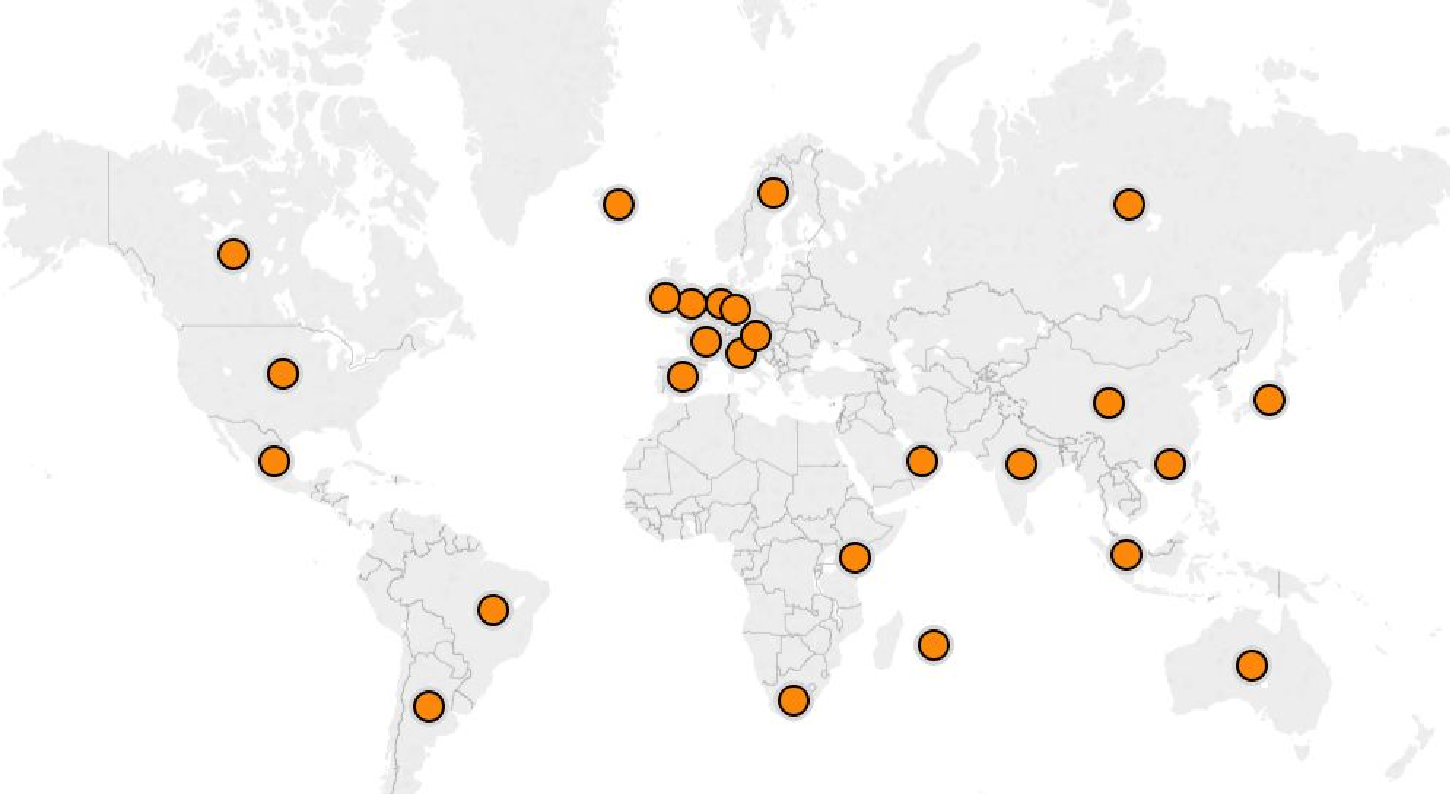
\includegraphics[width=0.8\columnwidth]{World-DNS}
%\caption{Vantage points in measuring hosting diversity.}
%\label{fig:world}
%\end{figure}

\begin{figure}[t]
\centering
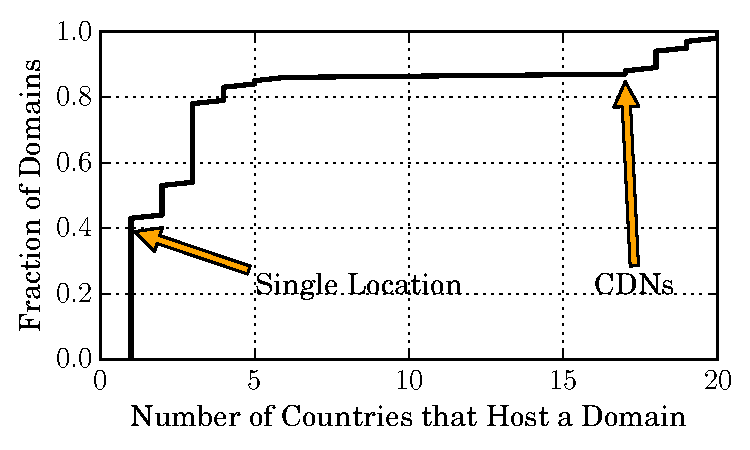
\includegraphics[width=.8\columnwidth]{domain_hist_US1}
\caption{The number of Alexa Top 100 US Domains hosted in different countries.}
\label{fig:host_diversity}
\end{figure}


\begin{figure*}[t!]
\begin{minipage}{\linewidth}
\begin{subfigure}[b]{.32\linewidth}
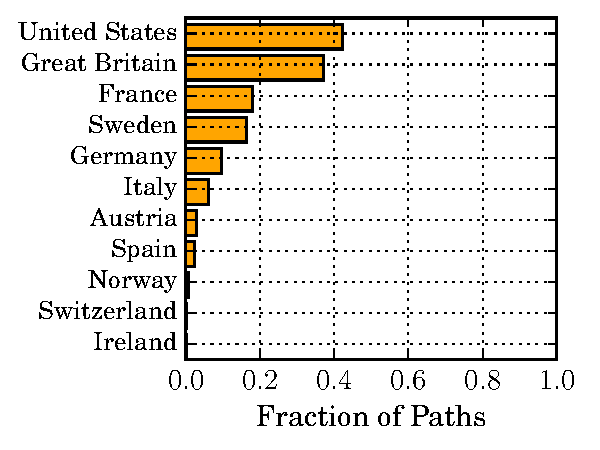
\includegraphics[width=\linewidth]{nl_trombone_new11}
\caption{The Netherlands.\label{fig:trombone_netherlands}}
\end{subfigure}
\begin{subfigure}[b]{.32\linewidth}
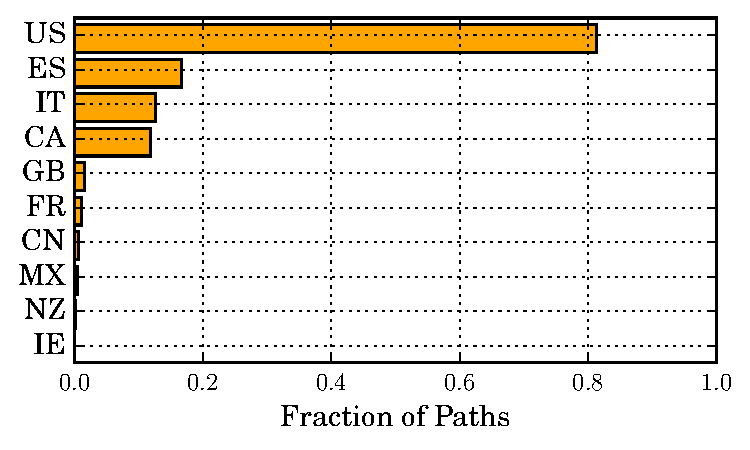
\includegraphics[width=\linewidth]{br_trombone_new11}
\caption{Brazil.\label{fig:trombone_brazil}}
\end{subfigure}
\begin{subfigure}[b]{.32\linewidth}
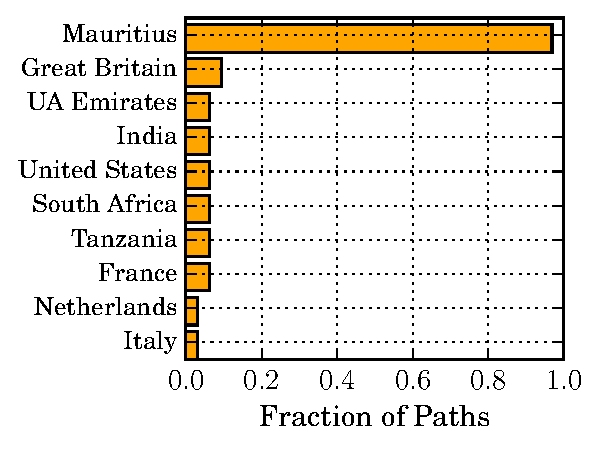
\includegraphics[width=\linewidth]{ke_trombone_new11}
\caption{Kenya.\label{fig:trombone_kenya}}
\end{subfigure}
\end{minipage}
\caption{The countries that tromboning paths from the Netherlands, Brazil, and Kenya transit.}
\label{fig:trombone}
\end{figure*}



\begin{finding}[Domain Hosting]
The most common destination, regardless of originating country, is the United States.
\end{finding}
\noindent
Table~\ref{tab:host} shows the fraction of paths that are hosted in various
countries.  Despite the extent of country-level hosting diversity, the
majority of paths from all of the countries we studied terminate in a single
country; 77\%, 45\%, 63\%, 44\%, and 97\% of paths originating in Brazil, Netherlands, India,
Kenya, and the United States, respectively, are currently reaching content located in the
United States.   Our results also
show the Netherlands is a common hosting location for paths originating in the
Netherlands, India, and Kenya.

%For Indian traffic, in addition to the 63\% hosted in the United States and the 10\% hosted in the Netherlands, another 10\% is hosted in Singapore.  Hosting in these countries can best be explained by the number of underwater cables with landing points in both India and Singapore~\cite{cablemap}.  More specifically, there is a cable that directly connects Chennai, India and Changi North, Singapore, and is owned by Tata Communications, which is one of the top global Internet providers (in terms of transited IP space)~\cite{bakers}.  

%For Kenyan traffic, the United States hosts 44\% of the content, but Ireland hosts 10\%; Ireland is a popular hosting location for U.S. companies due to its relaxed enforcement of privacy in the private sector \annie{I got this information from Joel Reidenberg - how do I cite that?  I'll also look to see if I can find any publications that discuss this}.  

\begin{finding}[Domestic Traffic]
All of the countries we studied (except for the United States) host content for a small percentage of the paths that originate in their own country; they also host a small percentage of their respective country-code top-level domains.
\end{finding}
\noindent
Only 17\% of paths that originate in Brazil also end there, and only 5\%
and 2\% of Indian and Kenyan paths, respectively, end in the originating
country.  
For Kenya, 24 out of the Top 100 Domains are .ke domains, but only 5
of the 24 are hosted within Kenya.  29 out of 40 .nl domains are hosted in the Netherlands;
four of 13 .in domains are hosted in India; 18 of 39 .br domains are hosted in Brazil.  
Figure \ref{fig:cctld_graph} shows these results.  As one might expect, all .gov domains were hosted in their respective country. 

\begin{figure}[t]
\centering
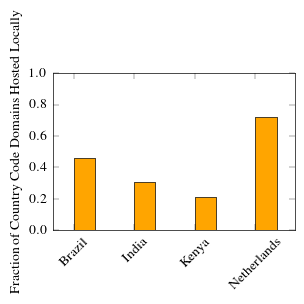
\includegraphics[width=.4\textwidth]{compare_cctld}
\caption{Fraction of country code top-level domains that are hosted locally.}
\label{fig:cctld_graph}
\end{figure}

\begin{finding}[Transit Traffic]
The United States and Great Britain are on the largest portion of paths in comparison to any other (foreign) country.
\end{finding}
\noindent
84\% of Brazilian paths traverse the United States, despite Brazil's
strong efforts to avoid United States surveillance~\cite{brazil_break_from_US,brazil_us_companies,brazil_conference,brazil_conference2,brazil_human_rights,brazil_cable}.  Although India and
Kenya are geographically distant, 72\% and 62\% of their paths also transit
the United States.

Great Britain and the Netherlands are on 
many of the paths from Kenya and India:
50\% and 20\% of
paths that originate in Kenya and India, respectively, transit Great
Britain.   Many paths likely traverse Great Britain and the Netherlands due to
the presence of large Internet Exchange Points (\ie, LINX, AMS-IX).
Mauritius, South Africa, and the United Arab Emirates transit 32\%,
33\%, and 15\% of paths from Kenya.  There are direct underwater cables
from Kenya to Mauritius, and from Mauritius to South
Africa~\cite{cablemap}.



\begin{finding}[Tromboning Traffic]
Brazilian and Netherlands paths often trombone to the United States, despite the prevalence of IXPs in both countries.
\end{finding}
\noindent
Figure~\ref{fig:trombone}
shows the fraction of paths that trombone to
different countries for the Netherlands, Brazil, and Kenya. 24\% of
all paths originating in the Netherlands (62\% of domestic paths)
trombone to a foreign country before returning to the
Netherlands. Despite Brazil's strong efforts in building IXPs to keep
local traffic local, 
their paths still trombone to the U.S.  This is due to IXPs being seen
as a threat by competing commercial providers; providers are sometimes
concerned that interconnection will result in making business
cheaper for competitors and stealing of customers~\cite{ixp_policy}.

Brazilian providers likely see one another as competitors and therefore as a
threat at IXPs, which causes them to peer with international providers instead
of other local providers.  Additionally, we see Brazilian paths trombone to
Spain and Italy.  We see Italy often in tromboning paths because Telecom
Italia Sparkle is one of the top global Internet providers~\cite{bakers}. 
MaxMind's geolocation sometimes mislabels IP addresses to be in
Spain when they are actually located in Portugal.  Despite our inability to
disambiguate Spain and Portugal, some of the issues associated with tromboning,
such as performance, are still pertinent. We are not aware of specific laws in
either of these countries that would make this distinction important from a
policy or legal aspect, either.

Tromboning paths that originate in Kenya most commonly traverse Mauritius,
which is expected considering the submarine cables between Kenya and
Mauritius.  Additionally, a cable from Mombasa,
Kenya to Fujairah, United Arab Emirates likely explains why many
paths include these countries. 

  %Traffic that should be kept local is susceptible to surveillance because it transits two well-known surveillance states.  

\begin{finding}[United States as an Outlier]
The United States hosts 97\% of the content that is accessed from within the United States, and only five foreign countries---France, Germany, Ireland, Great Britain, and the Netherlands---host content for the other 3\% of paths.
\end{finding}
\noindent

We find that Brazilian, Dutch, Indian, and Kenyan paths
often transit the U.S. The results from
studying paths that originate in the United States are drastically different from
those
of the other four countries.  The majority of locally popular content in these countries
is hosted outside of the respective country, which is shown in Table~\ref{tab:host}; in contrast, the United States hosts
97\% of the
content that is accessed from within the country.  Only 13 unique countries
are ever on a path from the United States to a domain in the top 100 (or third party
domain), whereas 30, 30, 25, and 38 unique countries are seen on the paths
originating in Brazil, Netherlands, India, and Kenya, respectively.

%There are only 6 foreign countries---France, Germany, Ireland, Great Britain, and the Netherlands----that host content for traffic originating in the United States, and the fraction of content hosted in these countries is less than 4\% combined.

\subsection{Limitations}

This section discusses the various limitations of our measurement methods
and how they may affect our results.

\paragraph{Traceroute accuracy and completeness}
Our study is limited by the accuracy and completeness of traceroute.
Anomalies can occur in traceroute-based
measurements~\cite{augustin2006avoiding}, but most traceroute anomalies
do not cause an overestimation in states that manipulate or monitor traffic.  The
incompleteness of traceroutes, where a router does not respond, causes
our results to underestimate the number of states that interfere with network 
traffic.

\paragraph{IP geolocation vs.\ country mapping}
There are fundamental challenges in deducing a geographic location
from an IP address, 
%JEN: remove the details about methods?
despite using different methods such as DNS names of the target,
network delay measurements, and host-to-location mapping in
conjunction with BGP prefix
information~\cite{padmanabhan2001investigation}.  While there are
inaccuracies and incompleteness in MaxMind's
data~\cite{huffaker2011geocompare}, the primary motivations for this work are to show that paths 
are currently going through countries with controversial policies on network interference, and that performance is affected by the 
paths taken.  
%We use Maxmind to map IP to country,
% (as described in Section~\ref{c_map}),
%which provides a lower
%bound on the amount of surveillance and tromboning.

\paragraph{IPv4 vs.\ IPv6 connectivity}
We collect and analyze only IPv4 paths.  IPv6 paths likely
differ from IPv4 paths as not all routers that support IPv4 also support
IPv6.  A comparable study of IP-level paths is an avenue for future work.

